\section{PAGE NUMBERING}
    
Please do \textbf{not} paginate your paper. Page numbers and conference identification will be inserted when the paper is included in the proceedings.
\pagebreak
	
\section{Illustrations, graphs, photographs and tables}
	
Illustrations must appear within the designated margins. If needed, figures may span the two columns. If possible, position illustrations at the top of columns, rather than in the middle or at the bottom. Caption and number every illustration (Figure \ref{example_figure}). The same rules apply to tables (Table \ref{example_table}). 
	
\begin{figure}[h] % use [t] here to force figure to top
    \begin{center}
    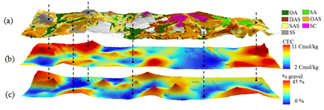
\includegraphics[width=\linewidth]{figures/example_figure.png}
    \caption{Figure caption (and also Table caption) must have a font 9 and be in bold.}
    \label{example_figure}
    \end{center}
\end{figure}

\begin{table}[h] % use [t] here to force table to top
    \centering
    \begin{tabular}{|c|c|c|c|}
        \hline
        \textbf{Item 1} & \textbf{Item 2} & \textbf{Item 3} & \textbf{Item 4}  \\
        \hline
        Value 11 & Value 12 & Value 13 & Value 14  \\
        \hline
        Value 21 & Value 22 & Value 23 & Value 24  \\
        \hline
    \end{tabular}
    \caption{Rules for table caption are the same as figures.}
    \label{example_table}
\end{table}
